% Options for packages loaded elsewhere
\PassOptionsToPackage{unicode}{hyperref}
\PassOptionsToPackage{hyphens}{url}
\PassOptionsToPackage{dvipsnames,svgnames,x11names}{xcolor}
%
\documentclass[
  letterpaper,
  DIV=11,
  numbers=noendperiod]{scrartcl}

\usepackage{amsmath,amssymb}
\usepackage{iftex}
\ifPDFTeX
  \usepackage[T1]{fontenc}
  \usepackage[utf8]{inputenc}
  \usepackage{textcomp} % provide euro and other symbols
\else % if luatex or xetex
  \usepackage{unicode-math}
  \defaultfontfeatures{Scale=MatchLowercase}
  \defaultfontfeatures[\rmfamily]{Ligatures=TeX,Scale=1}
\fi
\usepackage{lmodern}
\ifPDFTeX\else  
    % xetex/luatex font selection
\fi
% Use upquote if available, for straight quotes in verbatim environments
\IfFileExists{upquote.sty}{\usepackage{upquote}}{}
\IfFileExists{microtype.sty}{% use microtype if available
  \usepackage[]{microtype}
  \UseMicrotypeSet[protrusion]{basicmath} % disable protrusion for tt fonts
}{}
\makeatletter
\@ifundefined{KOMAClassName}{% if non-KOMA class
  \IfFileExists{parskip.sty}{%
    \usepackage{parskip}
  }{% else
    \setlength{\parindent}{0pt}
    \setlength{\parskip}{6pt plus 2pt minus 1pt}}
}{% if KOMA class
  \KOMAoptions{parskip=half}}
\makeatother
\usepackage{xcolor}
\ifLuaTeX
  \usepackage{luacolor}
  \usepackage[soul]{lua-ul}
\else
  \usepackage{soul}
  
\fi
\setlength{\emergencystretch}{3em} % prevent overfull lines
\setcounter{secnumdepth}{-\maxdimen} % remove section numbering
% Make \paragraph and \subparagraph free-standing
\makeatletter
\ifx\paragraph\undefined\else
  \let\oldparagraph\paragraph
  \renewcommand{\paragraph}{
    \@ifstar
      \xxxParagraphStar
      \xxxParagraphNoStar
  }
  \newcommand{\xxxParagraphStar}[1]{\oldparagraph*{#1}\mbox{}}
  \newcommand{\xxxParagraphNoStar}[1]{\oldparagraph{#1}\mbox{}}
\fi
\ifx\subparagraph\undefined\else
  \let\oldsubparagraph\subparagraph
  \renewcommand{\subparagraph}{
    \@ifstar
      \xxxSubParagraphStar
      \xxxSubParagraphNoStar
  }
  \newcommand{\xxxSubParagraphStar}[1]{\oldsubparagraph*{#1}\mbox{}}
  \newcommand{\xxxSubParagraphNoStar}[1]{\oldsubparagraph{#1}\mbox{}}
\fi
\makeatother

\usepackage{color}
\usepackage{fancyvrb}
\newcommand{\VerbBar}{|}
\newcommand{\VERB}{\Verb[commandchars=\\\{\}]}
\DefineVerbatimEnvironment{Highlighting}{Verbatim}{commandchars=\\\{\}}
% Add ',fontsize=\small' for more characters per line
\usepackage{framed}
\definecolor{shadecolor}{RGB}{241,243,245}
\newenvironment{Shaded}{\begin{snugshade}}{\end{snugshade}}
\newcommand{\AlertTok}[1]{\textcolor[rgb]{0.68,0.00,0.00}{#1}}
\newcommand{\AnnotationTok}[1]{\textcolor[rgb]{0.37,0.37,0.37}{#1}}
\newcommand{\AttributeTok}[1]{\textcolor[rgb]{0.40,0.45,0.13}{#1}}
\newcommand{\BaseNTok}[1]{\textcolor[rgb]{0.68,0.00,0.00}{#1}}
\newcommand{\BuiltInTok}[1]{\textcolor[rgb]{0.00,0.23,0.31}{#1}}
\newcommand{\CharTok}[1]{\textcolor[rgb]{0.13,0.47,0.30}{#1}}
\newcommand{\CommentTok}[1]{\textcolor[rgb]{0.37,0.37,0.37}{#1}}
\newcommand{\CommentVarTok}[1]{\textcolor[rgb]{0.37,0.37,0.37}{\textit{#1}}}
\newcommand{\ConstantTok}[1]{\textcolor[rgb]{0.56,0.35,0.01}{#1}}
\newcommand{\ControlFlowTok}[1]{\textcolor[rgb]{0.00,0.23,0.31}{\textbf{#1}}}
\newcommand{\DataTypeTok}[1]{\textcolor[rgb]{0.68,0.00,0.00}{#1}}
\newcommand{\DecValTok}[1]{\textcolor[rgb]{0.68,0.00,0.00}{#1}}
\newcommand{\DocumentationTok}[1]{\textcolor[rgb]{0.37,0.37,0.37}{\textit{#1}}}
\newcommand{\ErrorTok}[1]{\textcolor[rgb]{0.68,0.00,0.00}{#1}}
\newcommand{\ExtensionTok}[1]{\textcolor[rgb]{0.00,0.23,0.31}{#1}}
\newcommand{\FloatTok}[1]{\textcolor[rgb]{0.68,0.00,0.00}{#1}}
\newcommand{\FunctionTok}[1]{\textcolor[rgb]{0.28,0.35,0.67}{#1}}
\newcommand{\ImportTok}[1]{\textcolor[rgb]{0.00,0.46,0.62}{#1}}
\newcommand{\InformationTok}[1]{\textcolor[rgb]{0.37,0.37,0.37}{#1}}
\newcommand{\KeywordTok}[1]{\textcolor[rgb]{0.00,0.23,0.31}{\textbf{#1}}}
\newcommand{\NormalTok}[1]{\textcolor[rgb]{0.00,0.23,0.31}{#1}}
\newcommand{\OperatorTok}[1]{\textcolor[rgb]{0.37,0.37,0.37}{#1}}
\newcommand{\OtherTok}[1]{\textcolor[rgb]{0.00,0.23,0.31}{#1}}
\newcommand{\PreprocessorTok}[1]{\textcolor[rgb]{0.68,0.00,0.00}{#1}}
\newcommand{\RegionMarkerTok}[1]{\textcolor[rgb]{0.00,0.23,0.31}{#1}}
\newcommand{\SpecialCharTok}[1]{\textcolor[rgb]{0.37,0.37,0.37}{#1}}
\newcommand{\SpecialStringTok}[1]{\textcolor[rgb]{0.13,0.47,0.30}{#1}}
\newcommand{\StringTok}[1]{\textcolor[rgb]{0.13,0.47,0.30}{#1}}
\newcommand{\VariableTok}[1]{\textcolor[rgb]{0.07,0.07,0.07}{#1}}
\newcommand{\VerbatimStringTok}[1]{\textcolor[rgb]{0.13,0.47,0.30}{#1}}
\newcommand{\WarningTok}[1]{\textcolor[rgb]{0.37,0.37,0.37}{\textit{#1}}}

\providecommand{\tightlist}{%
  \setlength{\itemsep}{0pt}\setlength{\parskip}{0pt}}\usepackage{longtable,booktabs,array}
\usepackage{calc} % for calculating minipage widths
% Correct order of tables after \paragraph or \subparagraph
\usepackage{etoolbox}
\makeatletter
\patchcmd\longtable{\par}{\if@noskipsec\mbox{}\fi\par}{}{}
\makeatother
% Allow footnotes in longtable head/foot
\IfFileExists{footnotehyper.sty}{\usepackage{footnotehyper}}{\usepackage{footnote}}
\makesavenoteenv{longtable}
\usepackage{graphicx}
\makeatletter
\def\maxwidth{\ifdim\Gin@nat@width>\linewidth\linewidth\else\Gin@nat@width\fi}
\def\maxheight{\ifdim\Gin@nat@height>\textheight\textheight\else\Gin@nat@height\fi}
\makeatother
% Scale images if necessary, so that they will not overflow the page
% margins by default, and it is still possible to overwrite the defaults
% using explicit options in \includegraphics[width, height, ...]{}
\setkeys{Gin}{width=\maxwidth,height=\maxheight,keepaspectratio}
% Set default figure placement to htbp
\makeatletter
\def\fps@figure{htbp}
\makeatother

\KOMAoption{captions}{tableheading}
\makeatletter
\@ifpackageloaded{caption}{}{\usepackage{caption}}
\AtBeginDocument{%
\ifdefined\contentsname
  \renewcommand*\contentsname{Table of contents}
\else
  \newcommand\contentsname{Table of contents}
\fi
\ifdefined\listfigurename
  \renewcommand*\listfigurename{List of Figures}
\else
  \newcommand\listfigurename{List of Figures}
\fi
\ifdefined\listtablename
  \renewcommand*\listtablename{List of Tables}
\else
  \newcommand\listtablename{List of Tables}
\fi
\ifdefined\figurename
  \renewcommand*\figurename{Figure}
\else
  \newcommand\figurename{Figure}
\fi
\ifdefined\tablename
  \renewcommand*\tablename{Table}
\else
  \newcommand\tablename{Table}
\fi
}
\@ifpackageloaded{float}{}{\usepackage{float}}
\floatstyle{ruled}
\@ifundefined{c@chapter}{\newfloat{codelisting}{h}{lop}}{\newfloat{codelisting}{h}{lop}[chapter]}
\floatname{codelisting}{Listing}
\newcommand*\listoflistings{\listof{codelisting}{List of Listings}}
\makeatother
\makeatletter
\makeatother
\makeatletter
\@ifpackageloaded{caption}{}{\usepackage{caption}}
\@ifpackageloaded{subcaption}{}{\usepackage{subcaption}}
\makeatother

\ifLuaTeX
  \usepackage{selnolig}  % disable illegal ligatures
\fi
\usepackage{bookmark}

\IfFileExists{xurl.sty}{\usepackage{xurl}}{} % add URL line breaks if available
\urlstyle{same} % disable monospaced font for URLs
\hypersetup{
  pdftitle={Teste de Page para k-amostras relacionadas},
  pdfauthor={Vitória Sesana},
  colorlinks=true,
  linkcolor={blue},
  filecolor={Maroon},
  citecolor={Blue},
  urlcolor={Blue},
  pdfcreator={LaTeX via pandoc}}


\title{Teste de Page para k-amostras relacionadas}
\author{Vitória Sesana}
\date{}

\begin{document}
\maketitle


\begin{verbatim}

Anexando pacote: 'dplyr'
\end{verbatim}

\begin{verbatim}
Os seguintes objetos são mascarados por 'package:stats':

    filter, lag
\end{verbatim}

\begin{verbatim}
Os seguintes objetos são mascarados por 'package:base':

    intersect, setdiff, setequal, union
\end{verbatim}

Universidade Federal do Espírito Santo Centro de Ciências Exatas Curso
de Estatística Aplicada

Teste de Page para k-amostras relacionadas

Discente: Vitória N. de Jesus Sesana

Doscente: Dr.~Adelmo Inacio Bertolde

Vitória - ES 2025

\subsection{Sumário}\label{sumuxe1rio}

\begin{enumerate}
\def\labelenumi{\arabic{enumi}.}
\tightlist
\item
  Sobre o teste
\item
  Metodologia do teste
\item
  Aplicação prática com dados reais
\end{enumerate}

\section{Sobre o teste de page}\label{sobre-o-teste-de-page}

\subsection{História}\label{histuxf3ria}

A história do \textbf{Teste de Page} tem origem no contexto dos testes
não paramétricos desenvolvidos no século XX, e está associada ao
psicológo e estatístico americano \ul{Ellis Batten Page}, que propôs o
teste em 1963\footnote{Page, E. B. (1963). ``Ordered hypotheses for
  multiple treatments: a significance test for linear ranks.'' Journal
  of the American Statistical Association, 58(301), 216--230.}.

Elliot Page estava interessado em métodos eficientes para analisar dados
classificados (rankings), especialmente quando havia uma hipótese de
\textbf{ordem específica entre tratamentos}.

\subsection{Page x Friedman}\label{page-x-friedman}

Ao contrário do teste friedman para k-amostras relacionadas, o teste de
page considera a ordinalidade dos dados para cada bloco.

Ou seja, ele é uma extensão do teste de Friedman, mas com uma hipótese
alternativa ordenada, do tipo:

\[ \text{Tratamento 1} \leq \text{Tratamento 2} \leq \dots \leq \text{Tratamento k}
\]

\begin{quote}
O teste de Page para alternativas ordenadas é ligeiramente mais poderoso
que a análise de variância de Friedman por postos.
\end{quote}

\subsection{Quando usar?}\label{quando-usar}

\begin{itemize}
\item
  Dados pareados ou em blocos.
\item
  As medições podem ser ordenadas (ordinais).
\item
  Quer verificar se existe uma tendência de ordenação entre os
  tratamentos.
\end{itemize}

\section{Metodologia}\label{metodologia}

\subsection{Dados}\label{dados}

\begin{longtable}[]{@{}
  >{\raggedright\arraybackslash}p{(\columnwidth - 8\tabcolsep) * \real{0.1304}}
  >{\raggedright\arraybackslash}p{(\columnwidth - 8\tabcolsep) * \real{0.2319}}
  >{\raggedright\arraybackslash}p{(\columnwidth - 8\tabcolsep) * \real{0.2319}}
  >{\raggedright\arraybackslash}p{(\columnwidth - 8\tabcolsep) * \real{0.1449}}
  >{\raggedright\arraybackslash}p{(\columnwidth - 8\tabcolsep) * \real{0.2609}}@{}}
\toprule\noalign{}
\begin{minipage}[b]{\linewidth}\raggedright
Bloco
\end{minipage} & \begin{minipage}[b]{\linewidth}\raggedright
Tratamento 1
\end{minipage} & \begin{minipage}[b]{\linewidth}\raggedright
Tratamento 2
\end{minipage} & \begin{minipage}[b]{\linewidth}\raggedright
\(\cdots\)
\end{minipage} & \begin{minipage}[b]{\linewidth}\raggedright
Tratamento \(k\)
\end{minipage} \\
\midrule\noalign{}
\endhead
\bottomrule\noalign{}
\endlastfoot
Bloco 1 & \(X_{1,1}\) & \(X_{1,2}\) & \(\cdots\) & \(X_{1,k}\) \\
Bloco 2 & \(X_{2,1}\) & \(X_{2,2}\) & \(\cdots\) & \(X_{2,k}\) \\
Bloco 3 & \(X_{3,1}\) & \(X_{3,2}\) & \(\cdots\) & \(X_{3,k}\) \\
\(\vdots\) & \(\vdots\) & \(\vdots\) & \(\ddots\) & \(\vdots\) \\
Bloco \(b\) & \(X_{b,1}\) & \(X_{b,2}\) & \(\cdots\) & \(X_{b,k}\) \\
\end{longtable}

\begin{quote}
Matriz com b blocos (linhas) e k tratamentos (colunas).
\end{quote}

\subsection[Passo a passo ]{\texorpdfstring{Passo a passo
\footnote{Código doi: 10.1080/01621459.1963.10500843}}{Passo a passo }}\label{passo-a-passo}

Passo a passo para a aplicação do teste:

\begin{enumerate}
\def\labelenumi{\arabic{enumi}.}
\tightlist
\item
  Obter a matriz de dados (blocos × grupo);
\item
  Rankear os dados dentro de cada linha;
\item
  Definir pesos conforme a ordem esperada;
\item
  Determinar o nível de confiança;
\item
  Calcular a estatística do teste;
\item
  Comparar com valor crítico ou usar aproximação normal para obter
  p-valor.
\end{enumerate}

\subsection{Hipóteses}\label{hipuxf3teses}

\[
\begin{cases}
H_0: \text{Não há tendência de ordenação entre os tratamentos} \\
H_1: \text{Existe uma tendência de ordenação específica entre os tratamentos}
\end{cases}
\]

Se você suspeita de uma tendência crescente \(T_{1} < \dots < T_{k}\),
então os pesos são:

\[w = \{1,\dots,k\}\]

E então suas hipóteses serão:

\[
\begin{cases}
H_0: \text{Não há tendência de ordenação entre os tratamentos} \\
H_1: T_{1} < \dots < T_{k}
\end{cases}
\]

\subsection{Estatística do teste}\label{estatuxedstica-do-teste}

\[ L = \sum{}_{j=1}^{k}w_{j}R_{j}\]

\begin{itemize}
\item
  \(w_{j}\) = peso esperado do tratamento j;
\item
  \(R_{j}\) = soma dos ranks do tratamento.\footnote{\(R_{j} =  \sum{}_{i=1}^{b}X_{ij}\)
    com \(i = {1,\dots,b}\) e \(j = {1,\dots,k}\)}
\end{itemize}

\subsection{Decisão}\label{decisuxe3o}

Você compara o valor de L com valores críticos em uma tabela de Page
(existe para pequenos valores de n e k), ou para maiores valores usa-se
a aproximação normal:

\[
\mu_L = \frac{n k (k+1)}{2}
\]

\[
\sigma_L^2 = \frac{n k (k+1)(2k+1)}{12}
\]

\[
Z = \frac{L - \mu_L}{\sigma_L}
\]

\subsection{Aplicação no R}\label{aplicauxe7uxe3o-no-r}

No pacote
\href{https://cran.r-project.org/web/packages/DescTools/DescTools.pdf}{DescTools},
há a seguinte função para executar o teste de page:

\begin{Shaded}
\begin{Highlighting}[]
\FunctionTok{library}\NormalTok{(DescTools)}
\FunctionTok{PageTest}\NormalTok{(dados)}
\end{Highlighting}
\end{Shaded}

Executa o Teste de Page para alternativas ordenadas usando um algoritmo
exato proposto por Stefan Wellek (1989) com dados em blocos não
replicáveis

\subsection{Função PageTest()}\label{funuxe7uxe3o-pagetest}

\begin{itemize}
\item
  A alternativa implementada é que o parâmetro de localização será
  crescente ao longo dos grupos. Se a direção oposta for necessária, a
  ordem dos grupos deve ser invertida dentro da matriz.
\item
  Os grupos e blocos são obtidos a partir dos índices das colunas e das
  linhas, respectivamente.
\item
  Valores NA não são permitidos nos grupos ou blocos; se y contiver NA,
  os blocos correspondentes serão removidos.
\item
  Para valores pequenos de k (métodos) ou N (objetos de dados), o
  PageTest calculará os valores-p exatos. Para k, N \textgreater{} 15,
  Inf, é retornada uma aproximação normal. Apenas um desses valores será
  retornado.
\end{itemize}

\section{Aplicação}\label{aplicauxe7uxe3o}

\subsection{Sobre os dados}\label{sobre-os-dados}

Foi aplicado um questionário para coletar a ordem de preferência de
alguns dos pratos principais não vegetarianos ofertados no
\textbf{Restaurante Universitário} da \emph{Universidade Federal do
Espírito Santo}.

Os pratos escolhidos foram: frango grelhado, peixe desfiado, carne
moída, nuggets e cozido misto.

O objetivo é verificar se as preferências dos estudantes seguem a
seguinte ordem:

\[ \text{Carne moída} <  \text{Cozido misto} <  \text{Frango grelhado} \\
\quad\;\;\; < \text{Peixe desfiado} < \text{Nuggets}\]

\subsection{Questionário}\label{questionuxe1rio}

\begin{enumerate}
\def\labelenumi{\arabic{enumi}.}
\tightlist
\item
  Você se considera vegano/vegetariano?

  \begin{itemize}
  \tightlist
  \item
    Sim/Não
  \end{itemize}
\item
  Quantas vezes por seman, em média, você frequenta o RU?

  \begin{itemize}
  \tightlist
  \item
    Nenhuma vez por semana;
  \item
    Raramente (1 vez por semana);
  \item
    Regularmente (2 a 5 vezes por semana);
  \item
    Frequentemente (6 a 10 vezes).
  \end{itemize}
\item
  Ranqueamento das opções de prato principal.
\end{enumerate}

\subsection{Ranqueamento}\label{ranqueamento}

\begin{center}
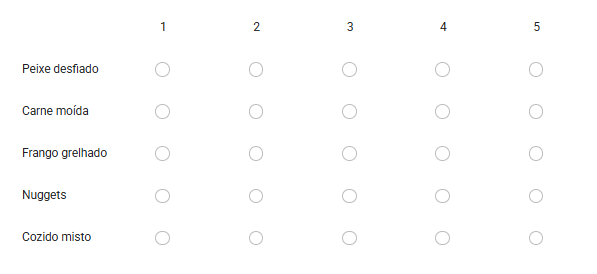
\includegraphics[width=0.5\textwidth,height=\textheight]{imagens/questionario.png}
\end{center}

\subsection{Hipóteses}\label{hipuxf3teses-1}

\begin{cases}
H_0: \text{Não há tendência de ordenação entre os tratamentos} \\
H_1: \text{Carne moída} <  \text{Cozido misto} <  \text{Frango grelhado} \\
\quad\;\;\; < \text{Peixe desfiado} < \text{Nuggets}
\end{cases}

Com os pesos sendo:

\[w = \{1,2,3,4,5\}\]

E o nível de signficância adotado:

\[\alpha = 5\%\]

\subsection{Análise exploratória dos
dados}\label{anuxe1lise-exploratuxf3ria-dos-dados}

\begin{itemize}
\item
  Quantidade total de estudantes: 30
\item
  Quantidade de vegetarianos/veganos:
\end{itemize}

\begin{longtable}[]{@{}ll@{}}
\toprule\noalign{}
Vegetariano/Vegano & Quantidade \\
\midrule\noalign{}
\endhead
\bottomrule\noalign{}
\endlastfoot
Sim & 0 \\
Não & 30 \\
Total & 30 \\
\end{longtable}

\subsection{Análise exploratória dos
dados}\label{anuxe1lise-exploratuxf3ria-dos-dados-1}

\begin{itemize}
\tightlist
\item
  Gráfico de barras das frequências semanais de idas ao RU:
\end{itemize}

\begin{verbatim}
Warning: The dot-dot notation (`..count..`) was deprecated in ggplot2 3.4.0.
i Please use `after_stat(count)` instead.
\end{verbatim}

\begin{center}
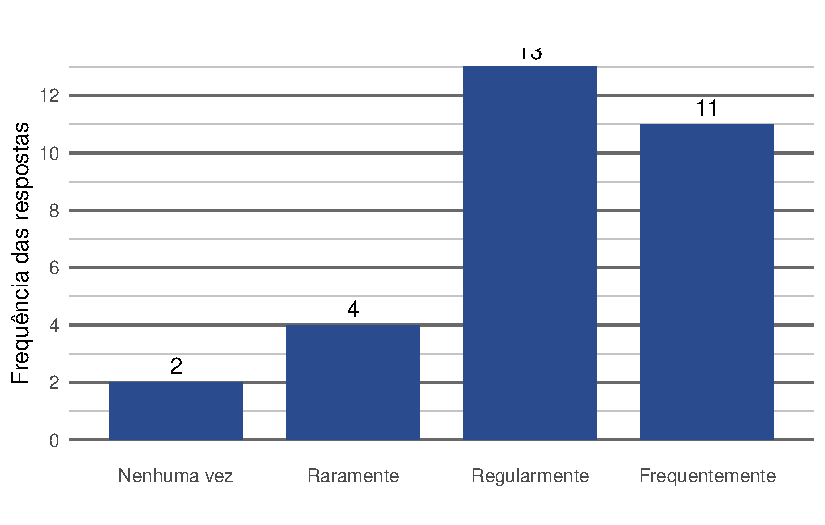
\includegraphics[width=0.75\textwidth,height=0.5\textheight]{PAGE-TEST-SLIDES_files/figure-pdf/unnamed-chunk-4-1.pdf}
\end{center}

\subsection{Análise exploratória dos
dados}\label{anuxe1lise-exploratuxf3ria-dos-dados-2}

\begin{itemize}
\tightlist
\item
  Percentual dos ranqueamentos por opção de prato principal:
\end{itemize}

\begin{center}
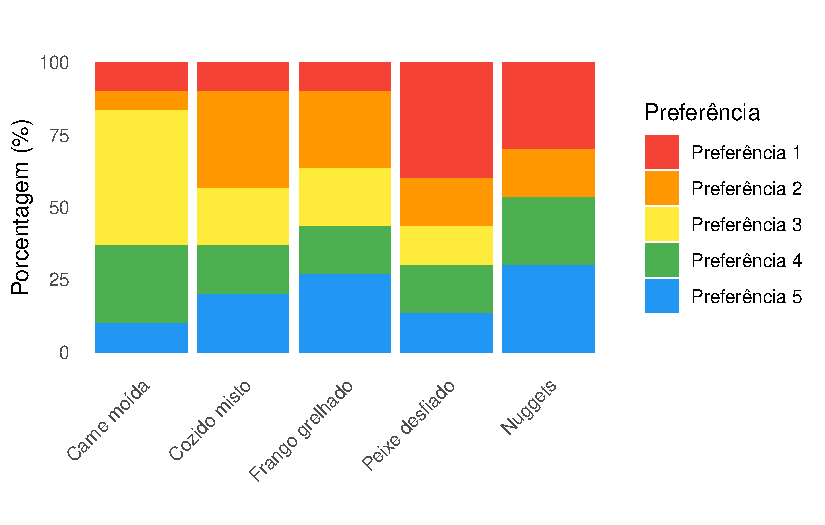
\includegraphics[width=0.9\textwidth,height=1\textheight]{PAGE-TEST-SLIDES_files/figure-pdf/unnamed-chunk-5-1.pdf}
\end{center}

\subsection{Aplicação do teste de
page}\label{aplicauxe7uxe3o-do-teste-de-page}

\begin{Shaded}
\begin{Highlighting}[]
\NormalTok{rankings }\OtherTok{\textless{}{-}} 
\NormalTok{  base }\SpecialCharTok{\%\textgreater{}\%} 
  \FunctionTok{select}\NormalTok{(}
\NormalTok{    carne\_moida, }
\NormalTok{    cozido\_misto,}
\NormalTok{    frango\_grelhado, }
\NormalTok{    peixe\_desfiado,}
\NormalTok{    nuggets,}
\NormalTok{  ) }\SpecialCharTok{\%\textgreater{}\%} 
  \FunctionTok{as.matrix}\NormalTok{()}

\FunctionTok{head}\NormalTok{(rankings)}
\end{Highlighting}
\end{Shaded}

\begin{verbatim}
     carne_moida cozido_misto frango_grelhado peixe_desfiado nuggets
[1,]           3            1               4              2       5
[2,]           3            1               2              4       5
[3,]           4            2               3              1       5
[4,]           3            2               5              1       4
[5,]           4            3               2              1       5
[6,]           2            4               1              3       5
\end{verbatim}

\subsection{Aplicação do teste de
page}\label{aplicauxe7uxe3o-do-teste-de-page-1}

\begin{Shaded}
\begin{Highlighting}[]
\FunctionTok{library}\NormalTok{(DescTools)}
\FunctionTok{PageTest}\NormalTok{(rankings)}
\end{Highlighting}
\end{Shaded}

\begin{verbatim}

    Page test for ordered alternatives

data:  rankings
L = 1325, p-value = 0.8235
\end{verbatim}

\subsection{Cenário 2}\label{cenuxe1rio-2}

Apenas indivíduos que vão frequentemente ao RU (6 a 10 vezes por
semana).

\begin{Shaded}
\begin{Highlighting}[]
\NormalTok{rankings\_2 }\OtherTok{\textless{}{-}} 
\NormalTok{  base }\SpecialCharTok{\%\textgreater{}\%} 
  \FunctionTok{filter}\NormalTok{(}
\NormalTok{    frequencia\_ru }\SpecialCharTok{\%in\%} \FunctionTok{c}\NormalTok{(}\StringTok{"Frequentemente"}\NormalTok{)}
\NormalTok{    ) }\SpecialCharTok{\%\textgreater{}\%} 
  \FunctionTok{select}\NormalTok{(}
\NormalTok{    carne\_moida, }
\NormalTok{    cozido\_misto,}
\NormalTok{    frango\_grelhado, }
\NormalTok{    peixe\_desfiado,}
\NormalTok{    nuggets,}
\NormalTok{  ) }\SpecialCharTok{\%\textgreater{}\%} 
  \FunctionTok{as.matrix}\NormalTok{()}

\FunctionTok{PageTest}\NormalTok{(rankings\_2)}
\end{Highlighting}
\end{Shaded}

\begin{verbatim}

    Page test for ordered alternatives

data:  rankings_2
L = 479, p-value = 0.8384
\end{verbatim}

\subsection{Referências}\label{referuxeancias}

Page, E. (1963): Ordered hypotheses for multiple treatments: A
significance test for linear ranks. Journal of the American Statistical
Association, 58, 216-230.

Siegel, S. \& Castellan, N. J. Jr.~(1988): Nonparametric statistics for
the behavioral sciences. Boston, MA: McGraw-Hill.

Wellek, S. (1989): Computing exact p-values in Page's nonparametric test
against trend. Biometrie und Informatik in Medizin und Biologie 20,
163-170

\url{https://cran.r-project.org/web/packages/DescTools/DescTools.pdf}

\section{Agradeço pela atenção!}\label{agradeuxe7o-pela-atenuxe7uxe3o}




\end{document}
